\documentclass{standalone}
\usepackage{tikz}
\usepackage{sansmath}

\usetikzlibrary{shapes.geometric,positioning,calc,petri,graphs}
\tikzset{
        node distance=1.5cm and 2.0cm,
        >=latex,
        font=\sf\bfseries\sansmath,
        ,
        textfeld/.style={align=center,minimum height=0.5cm,minimum width=1.5cm},
        pfeil/.style={->,line width=1.1pt},
        box/.style={rectangle,draw,line width=1.1pt,minimum height=1.5cm,minimum width=2.8cm,align=center},
        place/.style={circle,line width=1.1pt,draw=black,minimum size=6mm},
        transition/.style={rectangle,line width=1.1pt,draw=black,minimum size=6mm},
        every edge/.append style={line width=1.1pt}
        }
\tikzgraphsset{
    every graph/.style = {use existing nodes}
}

% \usetikzlibrary{arrows.meta,arrows,shapes,snakes,automata,backgrounds,,positioning,decorations.pathmorphing,backgrounds,fit}
% \tikzset{
%   node distance=1.25cm,
%   bend angle=45,
%   auto,
%   every picture/.style={/utils/exec={\sffamily}},
%   arrow/.style={-latex,thick},
%   inhibitor/.style={o-},
%   rtransition/.style={rectangle,very thick,draw=red,fill=red!30,minimum size=6mm},
%   btransition/.style={rectangle,very thick,draw=blue,fill=blue!30,minimum size=6mm},
%   -|/.style={to path={-| (\tikztotarget)}},
%   |-/.style={to path={|- (\tikztotarget)}},
%   }



\begin{document}
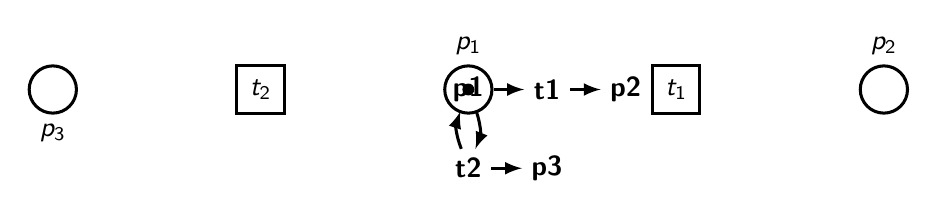
\begin{tikzpicture}
        \node[place,tokens=1,label=above:$ p_1 $] (p1) {};
        \node[transition] (t1) [right=of p1]{$ t_1 $};
        \node[place,label=above:$ p_2 $] [right=of t1](p2) {};
        \node[transition] (t2) [left=of p1]{$ t_2 $};
        \node[place,label=below:$ p_3 $] (p3) [left=of t2]{};
        \graph{
        p1 -> t1 -> p2,
        t2 ->[bend left=20] p1 ->[bend left=20] t2 -> p3
        };
\end{tikzpicture}
\end{document}